% book example for classicthesis.sty
\documentclass[
  oneside,
  12pt, a4paper,
  footinclude=true,
  headinclude=true,
  cleardoublepage=empty
]{scrbook}

\usepackage[linedheaders,parts,pdfspacing]{classicthesis}
\usepackage{mathtools, amsmath,amsfonts,amssymb, amsthm}
\usepackage{acronym}
\usepackage{geometry}
\usepackage{hyperref}
\usepackage[backend=bibtex,style=verbose-trad2]{biblatex}
\usepackage{float}
\usepackage{graphicx}
\usepackage{xargs}
\usepackage[colorinlistoftodos,prependcaption,textsize=tiny]{todonotes}
\newcommandx{\unsure}[2][1=]{\todo[linecolor=red,backgroundcolor=red!25,bordercolor=red,inline]{#2}}

\graphicspath{ {Figures/} }

\usepackage{tikz}
\usetikzlibrary{shapes,arrows}
\bibliography{refs}

\theoremstyle{definition}
\newtheorem{definition}{Definition}[section]

\theoremstyle{remark}
\newtheorem*{remark}{Remark}


\title{A decision support system for forecasting and optimal procurement}
\author{Neven Miculnic}

\begin{document}

\maketitle

% !TEX root = ../main.tex

%*******************************************************
% Abstract
%*******************************************************
\begin{abstract}
Optimal procurement in most industries involves forecasting of two
quantities: prices of raw materials and customer's demand.  The aim of
this work is to integrate forecasts into production planning models,
with the aim of minimizing overall procurement, holding and production
costs under demand satisfaction constraints.  The decision support
system should allow the decision maker to integrate qualitative,
unstructured information through a simple interface, for scenario
selection and solution refinement.


\keywords{procurement planning, dynamic lot sizing model, stochastic demands}
\end{abstract}

% !TEX root = ../main.tex

\chapter{Related Work}
\label{chap:Related Work}

\section{Newsvendor model}
\label{sec:Newsvendor model}

The newsvendor model~\autocite{Arrow1974} is a mathematical model resambling newsvendor stand. The problem is characterized by fixed prices and uncertain demand for a perishable product, e.g. yesterdays newspapers hold no value today. Demand for newspapers is uncertain and newsvendor must decide how many newspaper to buy for reselling.

The stock in newsvendor model is only for one day, and unlike problem presented in chapter~\ref{chap:prob-def} product is not perishable, but its cost increases in each following time step.

% !TEX root = ../main.tex

\chapter{Problem definition}
\label{chap:prob-def}
\section{introduction}

This problem is variation of lot sizing problem in stochastic setting. Variation is as follows. Firstly we describe deterministic variant before introducing stochasticity and uncertainty. We have predictions for raw material supply cost $\mathbf{s}$ at future time moment $t$. The \emph{factory} converts all bought raw materials at time $t$ and stores them into a warehouse. Number of discrete time moments is denoted by $n$.

One time moment storage costs fixed amount $h$, that is the holding cost.

Each $t$ we have certain demand we need satifying, denoted as $\mathbf{d}$. In case there's no products in storage to satisfy demand we pay backlogging cost denoted as $b$ per day, for late orders.

Our aim is to optimize our procurement policy by variating $\mathbf{x}$, that is product amount we buy at time moment $t$. However we are constrained by the maximum raw materials we can buy each day by $\mathbf{x_{\text{max}}}$.

\section{Formal problem definition}
\label{sec:Formal problem definition}

\subsection{Definitions}
\label{sub:Definitions}

Every input value is known beforehand, and it's assumed for random variables their distributions are known. Following is deterministic problem variant, and in subsequent chapters randomness and uncertainty is embedded into problem. Font convention:

\begin{align*}
x, y, z && \text{variables and constants} \\
\mathbf{x, y, z} && \text{vector variables and constants} \\
X, Y, Z && \text{random variables} \\
\mathbf{X, Y, Z} && \text{random vectors} \\
\mathcal{X, Y, Z} && \text{probability distributions} \\
\mathbf{A, B, C} && \text{matrices, by context differentiated from random vectors}
\end{align*}

Now following is formal problem description for deterministic variant:

\begin{align*}
    \mathbf{s} &= \begin{bmatrix}
        s_1, s_2, \dotsc, s_n
    \end{bmatrix}^\intercal && \text{Supply cost vector} \\
    \mathbf{x} &= \begin{bmatrix}
        x_1, x_2, \dotsc, x_n
    \end{bmatrix}^\intercal && \text{Procurement quantity vector} \\
    \mathbf{x_{\max}}  & && \text{Procurement quantity limits vector} \\
    \mathbf{d} &= \begin{bmatrix}
        d_1, d_2, \dotsc, d_n
    \end{bmatrix}^\intercal && \text{Demand random vector, $Y_t$ is a random variable} \\
    b & && \text{backlogging cost} \\
    h & && \text{holding cost}
\end{align*}

\subsection{Variables}
\label{sub:Variables}
$\mathbf{x}$ is our decision variable, as described previously.
\subsection{Constraints}
\label{sub:Constraints}
\begin{align*}
    \mathbf{x} &\in \mathbb{N}_0^n \\
    \mathbf{x} &\le \mathbf{x_{\text{max}}}\\
    \sum{x} &= \sum{d} \\
    b &\ge 0\\
    h &\ge 0\\
\end{align*}

\section{Objective function}

\begin{definition}{$c(t)$}
defines total speeding we pay at time $t$.
    \begin{equation}
        \label{eq:cost-t}
        c(t) = + s_t x_t + \begin{cases}
        h \left( \sum_{i=1}^t{x_i} - \sum_{i=1}^t{d_i} \right)  &
            \sum_{i=1}^t{x_i} \ge \sum_{i=1}^t{d_i}  \\
        b \left(\sum_{i=1}^t{d_i} - \sum_{i=1}^t{x_i} \right) &
            \sum_{i=1}^t{x_i} < \sum_{i=1}^t{d_i} \\
        \end{cases}
    \end{equation}
\end{definition}

\begin{definition}{$f(\mathbf{x})$}
    is objective function for this problem. Our aim is to minimize it.
    \begin{equation}
        f(\mathbf{x}) =  \sum_t{c(t)}
        \label{eq:cost-f}
    \end{equation}
\end{definition}

% !TEX root = ../main.tex

\chapter{Deterministic approach}
\label{chap:Deterministic approach}

\section{Modeling approaches}

Problem as defined in section~\ref{sec:prob-def} can be reduced to two well known problems: transportation and min-cost max flow problem. In both cases from knowledge of $\mathbf{x}$ and constraint equations, $\mathbf{x}^{(h)}$ and $\mathbf{x}^{(b)}$ since at each $t$ in optimal solution at least one of $x^{(b)}_t$ and $x^{(h)}_t$ is $0$. This fact can easily be observed from flow conservation on intermediate nodes as in fig~\ref{fig:mcmf-model}. Setting them both to positive values create positive flow cycle with positive cost, which can be canceled yielding same flow with lower cost.

\subsection{Reduction to transportation problem}
\label{subs:trans}

For transportation problem reduction we need cost matrix for satisfying demand at time $j$ with supply at time $i$. It is given as follows:

\begin{definition}{$\mathbf{C}$}
matrix defines cost for satisfying demand with specific raw supply material purchase date. It's element $c_{ij}$ equals:

\begin{equation*}
    c_{ij} = \begin{cases}
        b \left( i - j \right) + s_i & j < i \\
        h \left( j - i \right) + s_i & j \ge i
    \end{cases}
\end{equation*}
That is using raw materials purchased at $i$ to satisfy demand at time $j$ incurs cost $c_{ij}$.
\end{definition}

Maximum supply $\mathbf{x^{(\max)}}$ is given, so is the demand vector $\mathbf{d}$. Since transportation problem required equal supply and demand nodes, we add a dummy demand node consuming excess supply.
\unsure{"That is 0 in the deterministic..." I don't understand what is the meaning of this remark and how can implement your feedback.}

Transportation problem~\autocite{or-textbook} is easy reduction since we have cost matrix $\mathbf{C}$ defining ``transportation'' costs associated with each possible assignment option. For successful reduction we only need adding dummy source or destination.

\subsection{Min cost max flow reduction}
\label{sub:Min cost max flow reduction}

We can exploit additional problem structure to achieve superior performance and modeling capabilities. In figure~\ref{fig:mcmf-model} we see network architecture.

\begin{figure}[h]
\label{fig:mcmf-model}
  \centering
  
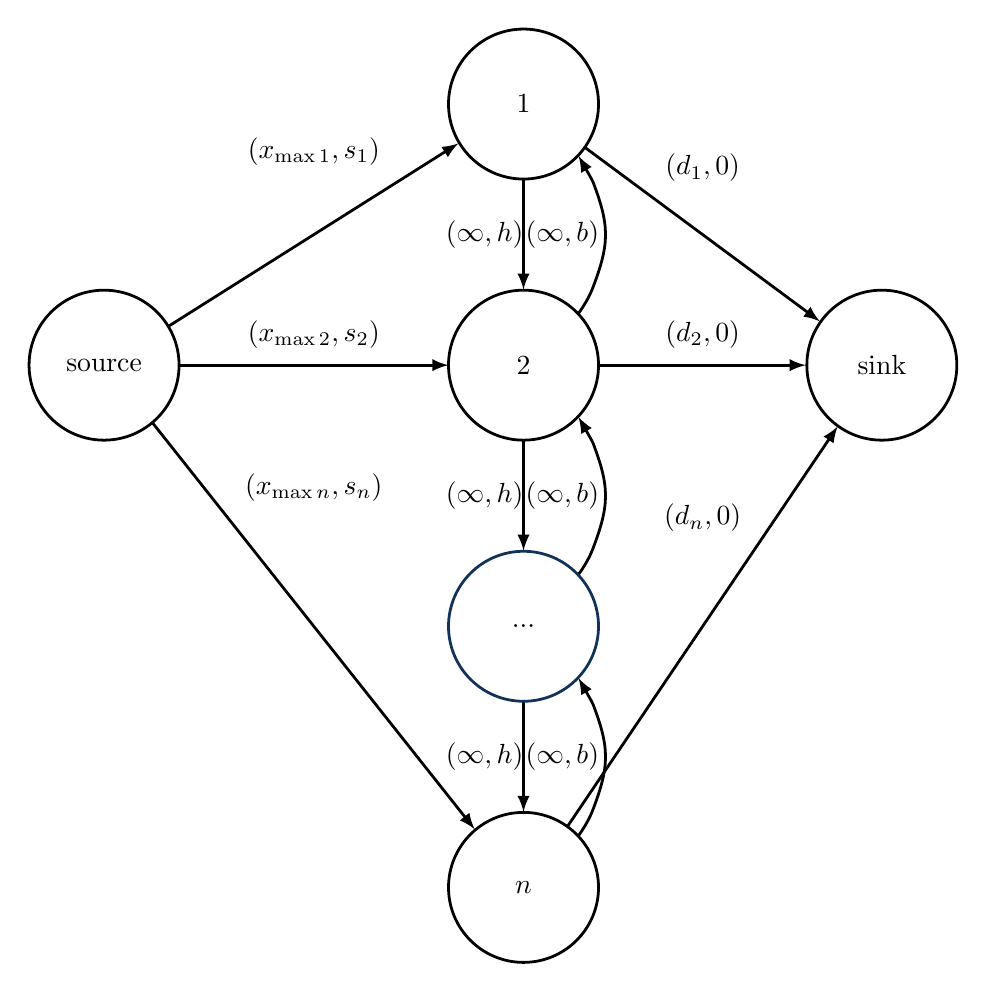
\begin{tikzpicture}[>=latex,line join=bevel,]
  \pgfsetlinewidth{1bp}
%%
\begin{scope}
  \pgfsetstrokecolor{black}
  \definecolor{strokecol}{rgb}{1.0,1.0,1.0};
  \pgfsetstrokecolor{strokecol}
  \definecolor{fillcol}{rgb}{1.0,1.0,1.0};
  \pgfsetfillcolor{fillcol}
  \filldraw (0.0bp,0.0bp) -- (0.0bp,336.0bp) -- (334.0bp,336.0bp) -- (334.0bp,0.0bp) -- cycle;
\end{scope}
\begin{scope}
  \pgfsetstrokecolor{black}
  \definecolor{strokecol}{rgb}{1.0,1.0,1.0};
  \pgfsetstrokecolor{strokecol}
  \definecolor{fillcol}{rgb}{1.0,1.0,1.0};
  \pgfsetfillcolor{fillcol}
  \filldraw (0.0bp,0.0bp) -- (0.0bp,336.0bp) -- (334.0bp,336.0bp) -- (334.0bp,0.0bp) -- cycle;
\end{scope}
  \pgfsetcolor{black}
  % Edge: n -> m
  \draw [->] (197.79bp,45.647bp) .. controls (199.91bp,48.565bp) and (201.75bp,51.712bp)  .. (203.0bp,55.0bp) .. controls (209.02bp,70.78bp) and (209.02bp,77.22bp)  .. (203.0bp,93.0bp) .. controls (202.92bp,93.205bp) and (202.84bp,93.41bp)  .. (197.79bp,102.35bp);
  \definecolor{strokecol}{rgb}{0.0,0.0,0.0};
  \pgfsetstrokecolor{strokecol}
  \draw (192.0bp,74.0bp) node {$(\infty, b)$};
  \draw (203.79bp,51.647bp) node {$$};
  \draw (203.79bp,96.353bp) node {$$};
  % Edge: m -> n
  \draw [->] (178.0bp,93.872bp) .. controls (178.0bp,84.622bp) and (178.0bp,74.113bp)  .. (178.0bp,54.189bp);
  \draw (164.0bp,74.0bp) node {$(\infty, h)$};
  \draw (184.0bp,90.872bp) node {$$};
  \draw (184.0bp,54.189bp) node {$$};
  % Edge: source -> 2
  \draw [->] (54.295bp,215.0bp) .. controls (78.339bp,215.0bp) and (114.12bp,215.0bp)  .. (150.97bp,215.0bp);
  \draw (102.5bp,226.0bp) node {$(x_{\max 2}, s_2)$};
  \draw (60.295bp,209.0bp) node {$$};
  \draw (144.97bp,209.0bp) node {$$};
  % Edge: 2 -> 1
  \draw [->] (197.79bp,233.65bp) .. controls (199.91bp,236.57bp) and (201.75bp,239.71bp)  .. (203.0bp,243.0bp) .. controls (209.02bp,258.78bp) and (209.02bp,265.22bp)  .. (203.0bp,281.0bp) .. controls (202.92bp,281.21bp) and (202.84bp,281.41bp)  .. (197.79bp,290.35bp);
  \draw (192.0bp,262.0bp) node {$(\infty, b)$};
  \draw (203.79bp,239.65bp) node {$$};
  \draw (191.79bp,284.35bp) node {$$};
  % Edge: n -> sink
  \draw [->] (193.82bp,48.934bp) .. controls (216.41bp,82.381bp) and (259.56bp,146.25bp)  .. (291.08bp,192.92bp);
  \draw (242.5bp,160.0bp) node {$(d_n, 0)$};
  \draw (187.82bp,42.934bp) node {$$};
  \draw (285.08bp,186.92bp) node {$$};
  % Edge: m -> 2
  \draw [->] (197.79bp,139.65bp) .. controls (199.91bp,142.57bp) and (201.75bp,145.71bp)  .. (203.0bp,149.0bp) .. controls (209.02bp,164.78bp) and (209.02bp,171.22bp)  .. (203.0bp,187.0bp) .. controls (202.92bp,187.21bp) and (202.84bp,187.41bp)  .. (197.79bp,196.35bp);
  \draw (192.0bp,168.0bp) node {$(\infty, b)$};
  \draw (203.79bp,145.65bp) node {$$};
  \draw (203.79bp,190.35bp) node {$$};
  % Edge: 2 -> m
  \draw [->] (178.0bp,187.87bp) .. controls (178.0bp,178.62bp) and (178.0bp,168.11bp)  .. (178.0bp,148.19bp);
  \draw (164.0bp,168.0bp) node {$(\infty, h)$};
  \draw (184.0bp,184.87bp) node {$$};
  \draw (184.0bp,148.19bp) node {$$};
  % Edge: 1 -> sink
  \draw [->] (200.26bp,293.27bp) .. controls (221.14bp,277.81bp) and (253.17bp,254.1bp)  .. (284.67bp,230.78bp);
  \draw (242.5bp,286.0bp) node {$(d_1, 0)$};
  \draw (206.26bp,287.27bp) node {$$};
  \draw (278.67bp,224.78bp) node {$$};
  % Edge: 1 -> 2
  \draw [->] (178.0bp,281.87bp) .. controls (178.0bp,272.62bp) and (178.0bp,262.11bp)  .. (178.0bp,242.19bp);
  \draw (164.0bp,262.0bp) node {$(\infty, h)$};
  \draw (184.0bp,281.87bp) node {$$};
  \draw (184.0bp,245.19bp) node {$$};
  % Edge: source -> n
  \draw [->] (44.515bp,194.16bp) .. controls (71.142bp,160.57bp) and (123.63bp,94.338bp)  .. (160.41bp,47.931bp);
  \draw (102.5bp,171.0bp) node {$(x_{\max n}, s_n)$};
  \draw (50.515bp,188.16bp) node {$$};
  \draw (154.41bp,53.931bp) node {$$};
  % Edge: source -> 1
  \draw [->] (50.307bp,229.07bp) .. controls (75.653bp,245.06bp) and (117.2bp,271.27bp)  .. (154.54bp,294.83bp);
  \draw (102.5bp,292.0bp) node {$(x_{\max 1}, s_1)$};
  \draw (56.307bp,223.07bp) node {$$};
  \draw (148.54bp,288.83bp) node {$$};
  % Edge: 2 -> sink
  \draw [->] (205.01bp,215.0bp) .. controls (223.63bp,215.0bp) and (248.96bp,215.0bp)  .. (279.59bp,215.0bp);
  \draw (242.5bp,226.0bp) node {$(d_2, 0)$};
  \draw (211.01bp,209.0bp) node {$$};
  \draw (273.59bp,209.0bp) node {$$};
  % Node: m
\begin{scope}
  \definecolor{strokecol}{rgb}{0.07,0.2,0.34};
  \pgfsetstrokecolor{strokecol}
  \draw (178.0bp,121.0bp) ellipse (27.0bp and 27.0bp);
  \definecolor{strokecol}{rgb}{0.0,0.0,0.0};
  \pgfsetstrokecolor{strokecol}
  \draw (178.0bp,121.0bp) node {$...$};
\end{scope}
  % Node: n
\begin{scope}
  \definecolor{strokecol}{rgb}{0.0,0.0,0.0};
  \pgfsetstrokecolor{strokecol}
  \draw (178.0bp,27.0bp) ellipse (27.0bp and 27.0bp);
  \draw (178.0bp,27.0bp) node {$n$};
\end{scope}
  % Node: 1
\begin{scope}
  \definecolor{strokecol}{rgb}{0.0,0.0,0.0};
  \pgfsetstrokecolor{strokecol}
  \draw (178.0bp,309.0bp) ellipse (27.0bp and 27.0bp);
  \draw (178.0bp,309.0bp) node {$1$};
\end{scope}
  % Node: source
\begin{scope}
  \definecolor{strokecol}{rgb}{0.0,0.0,0.0};
  \pgfsetstrokecolor{strokecol}
  \draw (27.0bp,215.0bp) ellipse (27.0bp and 27.0bp);
  \draw (27.0bp,215.0bp) node {source};
\end{scope}
  % Node: 2
\begin{scope}
  \definecolor{strokecol}{rgb}{0.0,0.0,0.0};
  \pgfsetstrokecolor{strokecol}
  \draw (178.0bp,215.0bp) ellipse (27.0bp and 27.0bp);
  \draw (178.0bp,215.0bp) node {$2$};
\end{scope}
  % Node: sink
\begin{scope}
  \definecolor{strokecol}{rgb}{0.0,0.0,0.0};
  \pgfsetstrokecolor{strokecol}
  \draw (307.0bp,215.0bp) ellipse (27.0bp and 27.0bp);
  \draw (307.0bp,215.0bp) node {sink};
\end{scope}
%
\end{tikzpicture}


  \caption{min cost max flow model. Arcs are labeled (capacity, cost)}
\end{figure}

\subsection{Runtime complexity}

Since both transportation problem and min-cost max flow have polynomial solution algorithms~\autocite{or-textbook}~\autocite{Orlin1997}, this problem does too. Most efficient approach is using network simplex since this problem naturally fits into min-cost max flow model than reduction to transportation problem.

\section{Variants}
\label{sec:Variants}

Problem as defined previously could seem rather simplistic and not allowing useful extensions users might want, such as starting storage amount and similar. In following few subsections most useful extensions are described.

\subsection{Starting storage capacity}
In case we already have a certain number of product in stock we can easily embed that knowledge into the model by setting $x^{(h)}_0$ equal to starting storage capacity

\subsection{Ending storage requirement}
\label{subs:Ending storage requirement}
For example we'd like to have some extra product in stock by the end of analysis, and it's quite easy to accommodate such requirement. Simple set $x^{(h)}_n$ to ending requirements. In min-cost max flow model that would be equivalent to another arch from node $n$ to sink with ending storage requirement capacity.

\subsection{Allowing future backlogging}
\label{subs:Allowing future backlogging}
In the model as described, time stops at period $n$, however, in realistic scenario we're looking at only short time snapshot of ongoing process. Simplest modification would be allowing $x^{(b)}_n$ to be non-negative and letting it be decision variable. It's value is going to be amount of backlogged demand at the analysis end, that is time $n$.

\subsection{Leap time ordering}
\label{subs:leap-time-ordering}
If we order raw materials at $t$ they might arrive at later time moment $t+\Delta_t$. This can easily be modeled via variable substitution. For different $\Delta_t$ depending on the $t$ or multiple suppliers see Subsection~\ref{subs:Multiple raw material suppliers}

\subsection{Multiple raw material suppliers}
\label{subs:Multiple raw material suppliers}
Adding new raw material suppliers with different costs cannot be done as per original model specification. Talking in terms or min-cost max flow approach adding new raw material suppliers would be equal to adding additional arcs from source to nodes 1, 2, \ldots, $n$. with respective maximum supply capacity and costs.

% !TEX root = ../main.tex

\chapter{Deeper analysis}
\label{chap:Deeper analysis}

First we are going to analise problem deeply without presuming any independence or probability distribution on random variables. Later in subsequent chapters we are going to focus more on where demand at time $t$ has independent Gaussian distribution and mean.

\section{Cost function}
\begin{align*}
\shortintertext{The minimizing function is:}
    & \operatorname{E} \left[
        \mathbf{s}^\intercal\mathbf{x} + \sum{c(t)}
    \right] \\
\shortintertext{Due to linerality of expectation and $x$ being variable it's equal to:}
    & \mathbf{x} \operatorname{E} \left[
        \mathbf{s}^\intercal
        \right] +
        \operatorname{E} \left[ \sum{c(t)} \right] \\
\end{align*}

Therefore only needed modeling information for supply cost is its expectation $\operatorname{E} \left[ \mathbf{s} \right]$. The other part is more trickier since $D_i$ and $D_j$ aren't usually independent.

\section{Handling demand cost non-linearity}
\label{sec:Handling demand cost non-linearity}

As we can see in equation~\ref{eq:cost-t} we have non-linearity depending whether we're satifying all demand or are we backlogging demand at time $t$. Therefore here are two possible solutions for minimizing objective function~\ref{eq:cost-f}.

\subsubsection{Simulation}
\label{subs:Simulation}

We generate multiple scenarios for demand vector, $d$ according to probability distribution. For small $n$ and relatively small number of outcomes in each random variable we can exhaustedly model each scenario, scale it appropriately and feed to MIP solver\footnote{There's a trick on using binary variable for discontinuity in cost function~\ref{eq:cost-t}}

\subsubsection{Safety net approach}
\label{subs:Safety net approach}

Alternatively, we can artificially add new constraints and avoiding backlogging with arbitrary probably. This model assumes backlogging cost are significantly greater than storage cost, that is backlogging penalty is severe.

Thus we chose values $p_t$ which tell us the probabilit 

% !TEX root = ../main.tex

\chapter{Application on historical dataset}
\label{chap:Application on historical dataset}

For purpose of demonstrating for demand I'm using data from US electricity consumption~\autocite{us-elec} It offers per month aggregation of electrical energy used per state, and for purpose of illustration I'm using whole US aggregated. Data ranges from 1990 till February 2016. I'm using restricted version from 1990 till 2005 aggregated on yearly basis. Full data plot is in figure~\ref{fig:supply}

\begin{figure}[]
  \centering
  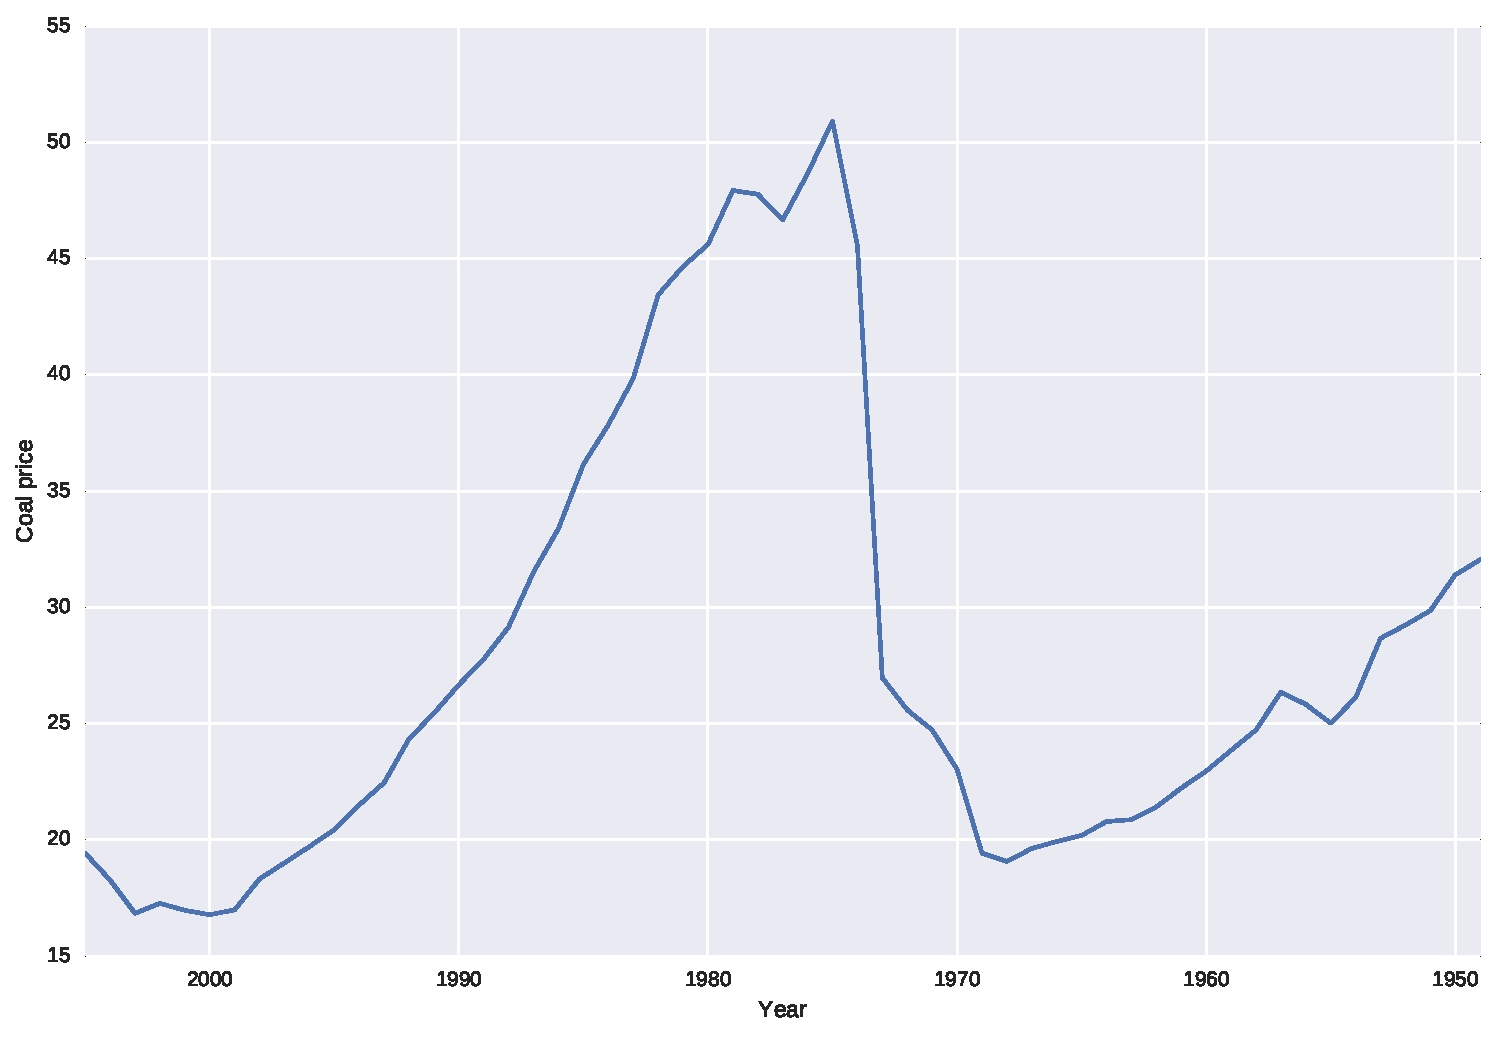
\includegraphics[width=0.8\linewidth]{supply}
  \caption{Yearly coal prices. Green are prediction with ARIMA(0,1,1) model}
  \label{fig:supply}
\end{figure}

For supply unit cost, for illustrative purposes I'm using historic American coal price~\autocite{us-coal}. It is yearly based from 1950 till 2005. The data is plot is in figure~\ref{fig:demand}.

First I'm going to compare optimal solution with perfect information to simple solution. Simple solution consists of buying current demand quantity each day from current day supply price. Planning is done on time horizon from 2000 till 2005. Later in this chapter ARIMA model is going to be fit to dataset and analysis be made. In table~\ref{my-label} you can see relative error of optimal solution versus simple approach for various holding and backlogging cost. On this particular dataset due to its simplistic nature more complicated optimal approach doesn't necessary bring much additional benefit. There's no silver bullet, but on more involved dataset profit gains are significant.

\begin{table}[]
\centering
\caption{Perfect information procurement}
\label{my-label}
\begin{tabular}{@{}llr@{}}
\toprule
$h$ & $b$ & relative error compared to optimal \\ \midrule
1   & 100 & 1.1\%          \\
1   & 10  & 1.1\%          \\
1   & 1   & 1.1\%          \\
10  & 1   & 0\%            \\
10  & 10  & 0\%            \\
100 & 1   & 0\%            \\ \bottomrule
\end{tabular}
\end{table}


For purposes of this analysis, data from 2000 till 2005 is going to be unknown and serve as demonstration of programming support helper functions. Whole programming support can be found at URL~\autocite{code}. Forecasting is done by fitting ARIMA model, where model selection is done with lowest Akaike information criterion~\autocite{Akaike1974}.

\begin{figure}[]
  \centering
  \includegraphics[width=0.8\linewidth]{demand}
  \caption{Yearly electricity demand. Green are predictions with ARIMA(1,2,0) model}
  \label{fig:demand}
\end{figure}

As we can see from figures~\ref{fig:demand} and~\ref{fig:supply}, automatic data forecasting yields subpar performance compared to true future data in both supply cost and in demand quantity time series. In supply it predicts decline in price, while the price is increasing, and in demand quantity it underestimates increase in demand.

Which is partially to be expected given model has only time series data as input, without all other world parameters influencing demand quantity and supply cost. For such cases expert opinions is of utmost importance and decision maker should decide which forecasted quantities make sense and which ones are underestimated/overestimated. Automatic approach works only for the most simplest cases, and knowledge of dedicated system or libraries would enable decision maker greater agility in implementing models, finding solutions and its refinement.

Despite mentioned shortcomings in this particular dataset, automatic method with backlogging cost $b=100$ and holding cost $h=1$, achieves 0.02\% accuracy for first step procurement quantity compared to ideal solution. Detailed jupyter notebook is located at URL~\autocite{jup}.


\printbibliography
\end{document}
